% \cleardoublepage

\newrefsection

\chapter{外文翻译: 在线带测试多处理器调度问题的随机算法}

论文标题:Randomized algorithms for fully online multiprocessor scheduling with testing

作者:Mingyang Gong等

\sectionnonum{摘要}

我们贡献了第一个随机化算法,该算法是任意多个确定性算法在完全在线多处理器调度与测试问题中的集成。
当只有两个机器时,我们展示了通过两个组件算法,其期望竞争比已经严格小于已证明的最佳确定性竞争比下界。
这种算法结果在文献中极为罕见。多处理器调度是最早得到大量研究的组合优化问题之一。
最近,多个研究小组研究了其测试变体,在该变体中,
每个作业 \( J_j \) 具有一个处理时间的上界 \( u_j \) 和一个长度为 \( t_j \) 的测试操作;
可以选择执行作业 \( J_j \) 的最大处理时间 \( u_j \),或者选择对 \( J_j \) 进行测试,
测试时间为 \( t_j \),以获得确切的处理时间 \( p_j \),然后立即执行该作业的 \( p_j \) 时间。
我们的目标问题是完全在线多处理器调度与测试问题,其中作业依次到达,
因此需要在作业到达时做出测试决策以及分配指定的机器。
我们首先利用 Yao 原理证明了至少三台机器情况下和仅两台机器情况下随机算法的期望竞争比下界分别为 1.6682 和 1.6522,
并提出了一个期望竞争比为 \( (\sqrt{\varphi' + 3} + 1)(\approx 3.1490) \)-竞争的随机算法,
该算法是通过一个非均匀概率分布集成了任意多个确定性算法,
其中 \( \varphi' = \frac{\sqrt{5}+1}{2} \) 是黄金比例。当只有两台机器时,
我们展示了基于两个确定性算法的随机化算法已经期望地 \( \frac{3\varphi + 3\sqrt{13 - 7\varphi}}{4}(\approx2.1839)\)-竞争,
同时证明了任何确定性算法的竞争比下界为 2.2117。\\
\textbf{关键词:} 调度问题;多处理器;带测试调度;完工时间;随机算法

\section{介绍}

我们在本文中研究完全在线的多处理器调度与测试问题~\cite{durr2018scheduling,durr2020adversarial,albers2021explorable,albers2021scheduling},
并从随机化算法的角度进行研究。多处理器调度~\cite{garey1979computers}是最早的已知 NP 难组合优化问题之一,在过去几十年中得到了广泛研究。多处理器调度的一个实例 \( I \) 包含一组 \( n \) 个作业 \( J = \{J_1, J_2, \dots, J_n\} \),每个作业都要在一组 \( m \) 台并行的相同机器 \( M = \{M_1, M_2, \dots, M_m\} \) 上非抢占地执行,目标是最小化最大完工时间 \( C_{\text{max}} \),即最大作业完成时间。与经典设置不同的是,在调度与测试中,每个作业 \( J_j \) 都有一个处理时间上界 \( u_j \),并且有一个长度为 \( t_j \) 的测试操作,但其处理时间 \( p_j \) 直到作业被测试后才会揭示。作业 \( J_j \) 可以在其中一台机器上执行 \( u_j \) 时间,或者选择先进行测试,测试时间为 \( t_j \),然后立即执行 \( p_j \) 时间。若所有作业都在时间零到达,则多处理器调度与测试是一个半在线问题,表示为 \( P | t_j, 0 \leq p_j \leq u_j | C_{\text{max}} \)。本文研究的是完全在线问题,其中作业按顺序到达,在作业到达时需要做出测试决策,并且指定测试和/或执行的机器,表示为 \( P | \text{online}, t_j, 0 \leq p_j \leq u_j | C_{\text{max}} \)。显然,半在线是完全在线的特例,在这两种情况下,调度器都应该利用已知的作业信息,在作业到达时决定是否进行测试,以便最好地平衡由于未知处理时间所消耗的总时间。

给定一个多项式时间的确定性算法,针对半在线或完全在线问题,令 \( C(I) \) 为该算法在实例 \( I \) 上产生的最大完工时间,而 \( C^*(I) \) 为最优离线调度的最大完工时间。算法的性能通过竞争比来衡量,定义为 \( \sup_I \{ C(I) / C^*(I) \} \),其中 \( I \) 遍历所有问题实例,算法称为 \( \sup_I \{ C(I) / C^*(I) \} \)-竞争的。切换到随机化算法时,我们相应地收集其在实例 \( I \) 上的期望最大完工时间 \( E[C(I)] \),该随机化算法称为 \( \sup_I \{ E[C(I)] / C^*(I) \} \)-竞争的。对于在线问题,随机化算法有时可以更好地处理不确定性,从而导致比最好的确定性算法更低的期望竞争比。我们为 \( P | \text{online}, t_j, 0 \leq p_j \leq u_j | C_{\text{max}} \) 提出了这样的一个随机化算法,并且进一步证明,当只有两台机器时,其期望竞争比严格小于任何确定性算法已证明的竞争比下界。

我们提醒读者,在我们的问题中,作业处理是非抢占的。
在文献中,研究人员还考虑了抢占式作业处理~\cite{durr2018scheduling,durr2020adversarial,albers2021explorable,albers2021scheduling},
其中任何测试或执行操作都可以被中断并稍后恢复,或者考虑了更为受限的测试抢占式变体~\cite{albers2021scheduling},在该变体中,已测试作业的测试和执行操作是非抢占的,但执行操作不必立即跟随测试操作,且不一定发生在同一台机器上。此外,我们的目标是最小化最大完工时间 \( C_{\text{max}} \),即最小最大目标;而另一个重要目标是最小化总作业完成时间,或者最小和目标,这也是受到了许多研究的关注~\cite{durr2018scheduling,durr2020adversarial,albers2021scheduling}。

\subsection{关于全在线问题的现有研究}

现有的针对完全在线问题 \( P | \text{online}, t_j, 0 \leq p_j \leq u_j | C_{\text{max}} \) 的近似算法,无论是确定性算法还是随机化算法,都不多。
我们首先区分一个特殊的情况,其中所有的测试操作时间均为单位时间,即对于每个作业 \( J_j \),有 \( t_j = 1 \),我们称之为均匀测试情况~\cite{durr2018scheduling,durr2020adversarial,albers2021scheduling},
表示为 \( P | \text{online}, t_j = 1, 0 \leq p_j \leq u_j | C_{\text{max}} \)。
注意,在一般的测试情况下,测试时间可以是任何非负值。
当只有一台机器时,机器上的作业处理顺序与最大完工时间无关。
这表明完全在线问题和半在线问题是相同的。第一组结果是关于半在线均匀测试问题 \( P_1 | t_j = 1, 0 \leq p_j \leq u_j | C_{\text{max}} \),
由 D¨urr 等人~\cite{durr2018scheduling,durr2020adversarial}提出。
他们提出,当 \( u_j \geq \varphi = \frac{\sqrt{5} + 1}{2} \) 时测试作业 \( J_j \),或者以概率 \( f(u_j) = \max \left( 0, \frac{u_j(u_j - 1)}{u_j(u_j - 1) + 1} \right) \) 测试它,
从而得到了一个确定性的 \( \varphi \)-竞争算法和一个期望的 4/3 竞争算法。
令 \( r_j = \frac{u_j}{t_j} \);Albers 和 Eckl~\cite{albers2021explorable}将上述两种算法扩展到一般测试情况下 \( P_1 | t_j, 0 \leq p_j \leq u_j | C_{\text{max}} \),
即当 \( r_j \geq \varphi \) 时测试作业 \( J_j \),或者以概率 \( f(r_j) \) 测试它,
分别达到了相同的竞争比和期望竞争比。作者们~\cite{durr2018scheduling,durr2020adversarial,albers2021explorable}证明了这两种算法是最优的,即 \( \varphi \) 是任何确定性算法的竞争比下界,
而 4/3 是任何随机化算法的期望竞争比下界,这一结果由 Yao 原理~\cite{yao1977probabilistic}得出。 

当至少有两台机器时,完全在线问题比半在线问题更为一般。Albers 和 Eckl~\cite{albers2021scheduling}提出了在列表调度规则~\cite{graham1966bounds}中测试作业 \( J_j \),即当 \( r_j \geq \varphi \) 时,按照该规则将每个作业分配到最空闲的机器上进行处理(可能是测试后执行)。他们证明了这样的算法是 \( \varphi(2 - \frac{1}{m}) \)-竞争的,且该分析是紧的,其中 \( m \) 是机器的数量。他们还证明了,即使在均匀测试情况下 \( P | \text{online}, t_j = 1, 0 \leq p_j \leq u_j | C_{\text{max}} \) 中,任何确定性算法的竞争比下界为 2~\cite{albers2021scheduling},并且对于两台机器的一般测试情况 \( P_2 | \text{online}, t_j, 0 \leq p_j \leq u_j | C_{\text{max}} \),即当只有两台机器时,其下界为 2.0953,这一结果也稍微更好~\cite{albers2021scheduling}。

\subsection{我们的成果}

对于完全在线和半在线的多处理器调度与测试问题,目标是最小化最大完工时间,我们已经看到,现有的随机化算法仅为单机器情况下的最优期望 \(\frac43\) 竞争算法~\cite{durr2018scheduling,durr2020adversarial,albers2021explorable}。
它们的期望竞争比严格小于任何确定性算法竞争比下界 \( \varphi \)。对于经典的在线多处理器调度问题,只有当 \( 2 \leq m \leq 5 \) 时,
Bartal 等人~\cite{bartal1992new} 和 Seiden~\cite{seiden2000online} 提出的算法的期望竞争比严格小于任何确定性算法的竞争比下界;
Albers~\cite{albers2002randomized} 提出的算法期望竞争比 1.916 也严格小于确定性下界 1.919,
但条件是只使用了三种离线最大完工时间下界。

在本文中,我们始终假设完全在线问题 \( P | \text{online}, t_j, 0 \leq p_j \leq u_j | C_{\text{max}} \) 中至少有两台机器。我们提出了一个几乎随机化的算法,它是任意多个组件确定性算法的集成,每个算法以一定的概率运行,并证明其期望竞争比最多为
\(
\sqrt{\left(1 - \frac{1}{m}\right)^2 \varphi^2 + 2\left(1 - \frac{1}{m}\right) + 1},
\)
其中 \( m \) 是机器的数量。这个期望竞争比随着 \( m \) 的增大而严格递增,严格小于 Albers 和 Eckl~\cite{albers2021scheduling}提出的最佳已知确定性算法的竞争比 \( \varphi(2 - \frac{1}{m}) \),并且当 \( m \) 趋于无穷大时,它逼近 \( (\sqrt{\varphi + 3} + 1) \approx 3.1490 \)。据我们所知,文献中的几乎随机化算法大多数是其组件确定性算法的均匀分布,而我们的算法则是第一个非均匀分布的任意多个组件算法。

当只有两台机器时,即对于 \( P_2 | \text{online}, t_j, 0 \leq p_j \leq u_j | C_{\text{max}} \),我们展示了在随机化算法中采用两个组件确定性算法导致的期望竞争比为
\(\dfrac{3\varphi + 3\sqrt{13 - 7\varphi}}{4} \approx 2.1839。\)

对于这个两台机器的情况,Albers 和 Eckl~\cite{albers2021scheduling} 证明了任何确定性算法的竞争比下界为 2.0953。
我们将其改进为 2.2117,从而证明我们的随机化算法在期望竞争比方面优于任何确定性算法。

\begin{figure}[t]
    \centering
    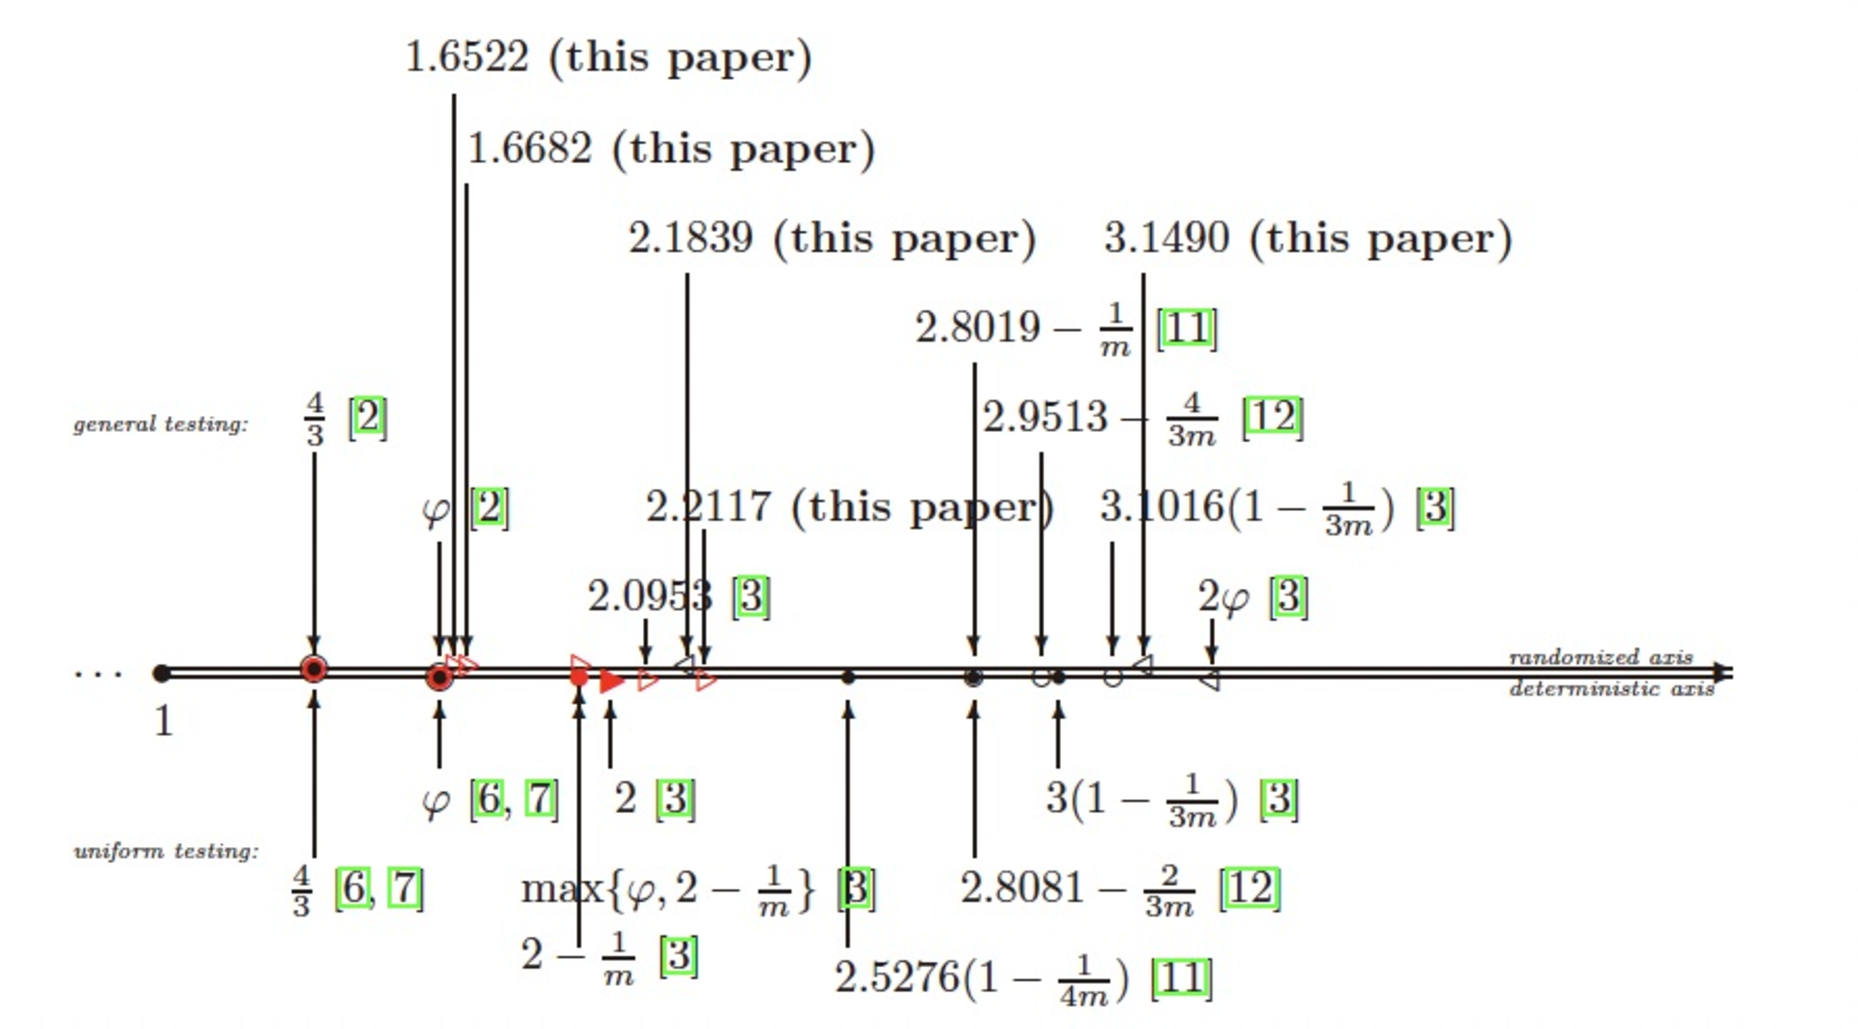
\includegraphics[width=.9\textwidth]{paper-results.pdf}
    \caption{现有的确定性和随机化算法在完全在线和半在线多处理器调度与测试问题中的竞争比。
    在横轴上,红色符号表示下界;三角形(\( \triangleleft \) 和 \( \triangleright \) 表示一般测试,否则表示均匀测试)
    表示完全在线问题的结果,而圆形(\(\circ\)表示一般测试,\(\cdot\)表示均匀测试)表示半在线问题的结果。
    在两个横轴之间,底部的轴表示确定性算法,顶部的轴表示随机化算法;
    轴上方的结果是针对一般测试情况的,而轴下方的结果是针对均匀测试情况的。
    }.
    \label{fig:paper-results}
\end{figure}

关于不可近似性,我们证明了至少三台机器时,任何随机化算法的期望竞争比下界为 1.6682,而在仅有两台机器时,对于 \( P_2 | \text{online}, t_j, 0 \leq p_j \leq u_j | C_{\text{max}} \),期望竞争比的下界为 1.6522,这两个下界都是使用稍微修改过的 Yao 原理~\cite{yao1977probabilistic} 得出的。
这两个下界在三台和两台机器情况下严格优于 Albers 和 Eckl~\cite{albers2021scheduling} 提出的下界 \( 2 - \frac{1}{m} \)。我们的所有结果总结如图~\ref{fig:paper-results}所示。

本文其余部分的组织结构如下:第 2 节介绍一些基本的符号和定义;接下来,在第 3 节中,我们证明了至少三台机器时完全在线问题 \( P | t_j, 0 \leq p_j \leq u_j | C_{\text{max}} \) 的期望竞争比下界 1.6682 和仅两台机器时的下界 1.6522;第 4 节包含了该问题的随机化算法及其性能分析、两台机器情况下稍微修改的随机化算法及其性能分析,以及对于 \( P_2 | \text{online}, t_j, 0 \leq p_j \leq u_j | C_{\text{max}} \) 的任何确定性算法的竞争比下界 2.2117;最后,第 5 节对论文进行了总结。

\section{预备内容}

我们研究完全在线的多处理器调度与测试问题,以最小化最大完工时间,记作 \( P | \text{online}, t_j, 0 \leq p_j \leq u_j | C_{\text{max}} \),其中作业依次到达。我们的目标是设计期望竞争比优于现有最先进的确定性算法的随机化算法,或者更进一步,优于已证明的最佳确定性竞争比下界。所有作业都在时间零到达的特殊情况称为半在线问题,记作 \( P | t_j , 0 \leq p_j \leq u_j | C_{\text{max}} \)。在适用的情况下,我们将证明半在线变体的下界。

多处理器调度与测试的一个实例 \( I \) 包含一组作业集 \( J = \{J_1, J_2, \dots, J_n\} \),每个作业都要在一组 \( m \) 台并行的相同机器 \( M = \{M_1, M_2, \dots, M_m\} \) 上执行,其中 \( n \) 和 \( m \geq 2 \) 是输入的一部分。每个作业 \( J_j \) 都有一个已知的处理时间上界 \( u_j \) 和一个长度为 \( t_j \) 的测试操作,处理时间 \( p_j \) 在测试操作执行之前是未知的。也就是说,调度器可以选择不测试作业 \( J_j \),而是执行它 \( u_j \) 时间,或者选择测试它 \( t_j \) 时间后,在同一台机器上立即执行 \( p_j \) 时间。

确定性算法 \( A \) 对是否测试作业做出二元决策。令 \( p_{A_j} \) 和 \( \rho_j \) 分别表示作业 \( J_j \) 在算法 \( A \) 和最优离线调度中的总时间。可以看到,当作业被测试时,\( p_{A_j} = t_j + p_j \),否则 \( p_{A_j} = u_j \),而 \( \rho_j = \min\{u_j, t_j + p_j\} \)。令 \( C_j \) 表示作业 \( J_j \) 在算法 \( A \) 生成的调度中的完成时间。问题的目标是最小化最大完工时间 \( C_{\text{max}} = \max_j C_j \)。我们使用 \( C_A(I) \)(当实例 \( I \) 在上下文中明确时,简称为 \( C_A \))和 \( C^*(I) \)(或相应的 \( C^* \))分别表示算法 \( A \) 和最优离线调度在实例 \( I \) 上的最大完工时间。

切换到更一般的随机化算法 \( A \),其在实例 \( I \) 上的期望最大完工时间表示为 \( E[C_A(I)] \)。

**定义 1(竞争比)**  
对于确定性算法 \( A \),竞争比是算法 \( A \) 生成的调度的最大完工时间与最优离线调度的最大完工时间之间的最坏情况比值,即

\[
\sup_I \left\{ \frac{C_A(I)}{C^*(I)} \right\}
\]

其中 \( I \) 遍历所有问题实例。对于更一般的随机化算法 \( A \),其期望竞争比为

\[
\sup_I \left\{ \frac{E[C_A(I)]}{C^*(I)} \right\}
\]

由于作业 \( J_j \) 的处理时间 \( p_j \) 可能达到 0 和 \( u_j \) 两个极端值,确定性算法通常会设置一个阈值函数 \( r_j = \frac{u_j}{t_j} \) 用于二元测试决策。直观上,随机化算法应该以概率 \( f(r_j) \) 测试作业 \( J_j \),并且该概率函数应该随着比率 \( r_j \) 的增大而增大,且当 \( r_j \leq 1 \) 时,\( f(r_j) = 0 \)。

实际上,D¨urr 等人 [6, 7] 和 Albers 与 Eckl [2] 在他们的最优期望 4/3 竞争随机化算法中使用了如下的概率函数:

\[
f(r) = 
\begin{cases}
0, & \text{如果 } r \leq 1, \\
\frac{r(r-1)}{r(r-1)+1}, & \text{如果 } r > 1.
\end{cases}
\]

他们分别应用于单机器问题 \( P_1 | \text{online}, t_j = 1, 0 \leq p_j \leq u_j | C_{\text{max}} \) 和 \( P_1 | \text{online}, t_j, 0 \leq p_j \leq u_j | C_{\text{max}} \)。遗憾的是,他们的成功不能轻易扩展到多机器情况,因为他们性能分析中使用的一个关键事实是,对于单台机器,期望最大完工时间等于所有作业期望处理时间的总和。我们在下面展示,对于多台机器,如果一个随机化算法使用式(1)中的概率函数来测试作业,那么当机器数量趋近于无穷大时,它的期望竞争比将是无界的。

\section{期望竞争下界}

\section{随机算法}

\section{结论}

\begingroup
    \linespreadsingle{}
    \printbibliography[title={外文翻译参考文献}]
\endgroup
